%%%%%%%%%%%%%%%%%%%%%%%%%%%%%%%%%%%%%%%%%
% Report
% LaTeX Template
% Version 1.0 (December 8 2014)
%
% This template has been downloaded from:
% http://www.LaTeXTemplates.com
%
% Original author:
% Brandon Fryslie
% With extensive modifications by:
% Vel (vel@latextemplates.com)
%
% License:
% CC BY-NC-SA 3.0 (http://creativecommons.org/licenses/by-nc-sa/3.0/)
%
%%%%%%%%%%%%%%%%%%%%%%%%%%%%%%%%%%%%%%%%%

\documentclass[usletter, 12pt]{article}
%%%%%%%%%%%%%%%%%%%%%%%%%%%%%%%%%%%%%%%%%
% Contract Structural Definitions File Version 1.0 (December 8 2014)
%
% Created by: Vel (vel@latextemplates.com)
% 
% This file has been downloaded from: http://www.LaTeXTemplates.com
%
% License: CC BY-NC-SA 3.0 (http://creativecommons.org/licenses/by-nc-sa/3.0/)
%
%%%%%%%%%%%%%%%%%%%%%%%%%%%%%%%%%%%%%%%%%

\usepackage{geometry} % Required to modify the page layout
\usepackage{multicol}
\usepackage{amsmath}
\usepackage{amssymb}

\usepackage[pdftex]{graphicx}
\usepackage{wrapfig}
\usepackage[font=scriptsize, labelfont=bf]{caption}
\usepackage[utf8]{inputenc} % Required for including letters with accents
\usepackage[T1]{fontenc} % Use 8-bit encoding that has 256 glyphs

\usepackage{avant} % Use the Avantgarde font for headings
\usepackage{courier}
\usepackage{xparse}
\usepackage{xcolor}
\usepackage{listings}  % for code verbatim and console outputs

\setlength{\textwidth}{16cm} % Width of the text on the page
\setlength{\textheight}{23cm} % Height of the text on the page
\setlength{\oddsidemargin}{0cm} % Width of the margin - negative to move text left, positive to move it right
\setlength{\topmargin}{-1.25cm} % Reduce the top margin

\setlength{\parindent}{0mm} % Don't indent paragraphs
\setlength{\parskip}{2.5mm} % Whitespace between paragraphs
\renewcommand{\baselinestretch}{1.5}

\definecolor{green}{rgb}{0.18, 0.55, 0.34}

\graphicspath{ {figures/} }
\captionsetup[table]{skip=10pt}

\lstset{language=C, keywordstyle={\bfseries \color{black}}}

% defines algorithm counter for chapter-level
\newcounter{nalg}[section]

%defines appearance of the algorithm counter
\renewcommand{\thenalg}{\thesection .\arabic{nalg}}

% defines a new caption label as Algorithm x.y
\DeclareCaptionLabelFormat{algocaption}{Algorithm \thenalg}

% defines the algorithm listing environment
\lstnewenvironment{pseudocode}[1][] {
    \refstepcounter{nalg}  % increments algorithm number
    \captionsetup{font=normalsize, labelformat=algocaption, labelsep=colon}
    \lstset{
        breaklines=true,
        mathescape=true,
        numbers=left,
        numberstyle=\scriptsize,
        basicstyle=\footnotesize\ttfamily,
        keywordstyle=\color{black}\bfseries,
        keywords={input, output, return, parallel, function, for, to, in, if,
        else, foreach, while, and, or, new, print},
        xleftmargin=.04\textwidth,
        #1
    }
}{}

\renewcommand{\familydefault}{\sfdefault}  % default font for entire document
  % document layout and style

% Member's information
\newcommand{\project}{Project 1: Divide and Conquer}
\newcommand{\members}{Sabbir Ahmed \& Zafar Mamarakhimov}

\begin{document}

    \begin{titlepage}

        \vspace*{\fill} % Add whitespace above to center the title page content
        \begin{center}

            {\LARGE \project~Analysis Report}\\ [1.5cm]

            \today
            
            \vspace*{\fill}

            \members

        \end{center}
        \vspace*{\fill} % Add whitespace below to center the title page content

    \end{titlepage}

    \section{Description}
    A recursive, divide-and-conquer algorithm was developed and analyzed to multiply together lists of complex numbers. Two different multiplication methods were used to compute the same products to analyze the crossover point.

        \subsection{Background}

        Multiplying two complex numbers are similar to multiplying polynomials. Let $z_{1}=x_{1}+iy_{1}$ and $z_{2}=x_{2}+iy_{2}$ be two complex numbers. Then their product is
            \[ z_{1}z_{2}=(x_{1}+iy_{1})(x_{2}+iy_{2})=(x_{1}x_{2}-y_{1}y_{2})+i(x_{1}y2+y_{1}x_{2}) \]

        The computation of a single complex product requires four real products and two real additions (subtraction is just addition with one operand negative and the "$+i$" does not count as an addition as this is really just notation to separate the real and imaginary parts).

        As it turns out, there is a way to reduce the number of real multiplications needed to compute a complex product.
            \[ (x_{1}+y_{1})(x_{2}+y_{2})=x_{1}x_{2}+(x_{1}y_{2}+y_{1}x_{2})+y_{1}y_{2} \]

        Let $t$ denote the product $(x_{1}+y_{1})(x_{2}+y_{2})$; then if the real products $r=x_{1}x_{2}$ and $s=y_{1}y_{2}$ are computed, the complex product is just
            \[ z_{1}z_{2}=(r-s)+i(t-r-s) \]

        Now, this computation only requires three real multiplications, but increases the number of additions to five. Since multiplication is the more expensive operation, it is expected for the reduction in the number of multiplies to pay-off, at least if the numbers are large enough.

        When multiplying a list of numbers, the difference between three or four real multiplications per complex multiplication can make a significant difference in the running time, especially if individual real multiplications are expensive.

    \section{Crossover Point}

        The point at which the asymptotically better algorithm becomes faster is known as the \textit{crossover point}.

        \subsection{Theoretical Results}
        Assume multiplication of two $b$-bit integers is $O(b^{2})$ and addition of two $b$-bit integers is $O(b)$.

        Consider, if $n = 2$, then computing the product of the list simply requires a single complex multiplication. For \texttt{cmul3()}, this means three multiplies of $b$-bit numbers, and five additions. There are some constants $c>0$ and $d>0$ such that the time to compute a $b$-bit multiply is bounded by $cb^2$ and the time for a $b$-bit addition is bounded by $db$.  Therefore, the time to multiply the two complex numbers, considering only multiplications and additions, is bounded by $3cb^2+5db$.

        \begin{figure}[ht]
            \begin{center}
                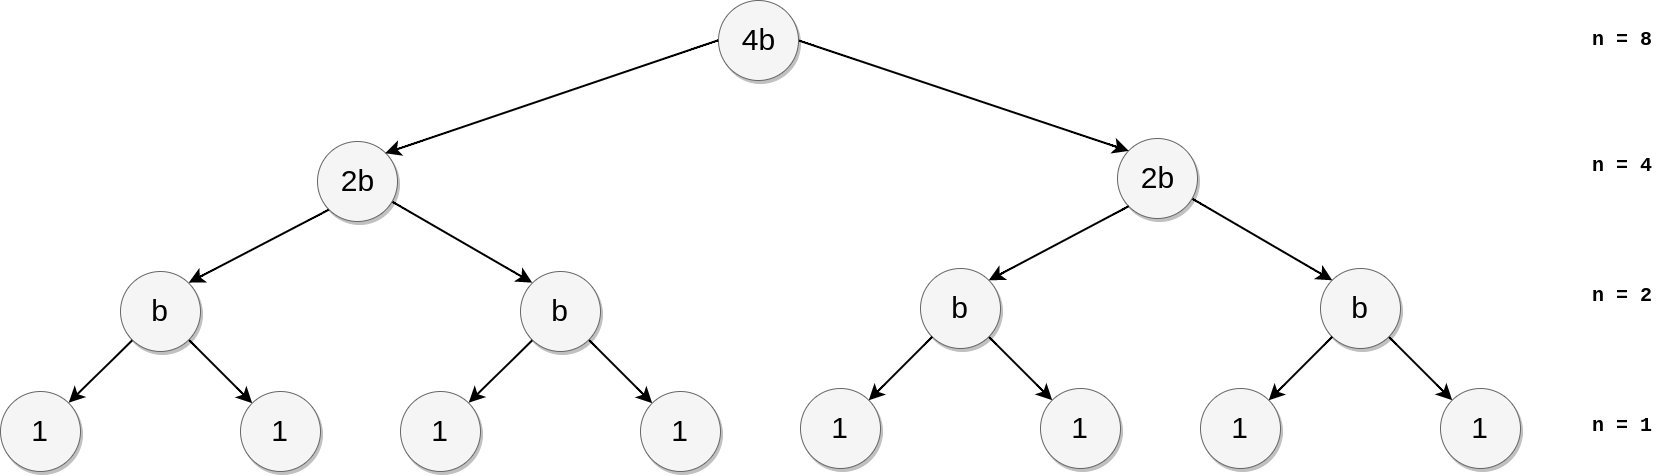
\includegraphics[width=1\textwidth]{multiplication_tree.png}
                \caption{Tree Visualization of the Divide and Conquer Method of Multiplication. $n$ is the Number of Integers Multiplied} \label{multiplication_tree}
            \end{center}
        \end{figure}

        According to the binary tree visualized, the number of bits grow by $\frac{n}{2}$, where $n$ is the total number of integers being multiplied. The recurrence relation may be derived from this method:

        \begin{equation*}
            \begin{split}
                f_1(n) & = 3c \Bigg( \frac{n}{2}b \Bigg)^2 + 5d \Bigg(\frac{n}{2}b \Bigg) \\
                & = \frac{3}{4}cb^2n^2+\frac{5}{2}dbn \\
            \end{split}
        \end{equation*}

        Similarly, for \texttt{cmul4()} would make four $b$-bit multiplies and two $b$-bit additions, so its running time is bounded by $4cb^2+2db$. The recurrence relation may be derived from this method:

        \begin{equation*}
            \begin{split}
                f_2(n) & = 4c \Bigg( \frac{n}{2}b \Bigg)^2 + 2d \Bigg(\frac{n}{2}b \Bigg) \\
                & = cb^2n^2+dbn \\
            \end{split}
        \end{equation*}

        Asymptotically, the runtime for either of the methods may be computed using the recurrence relation. Since the multiplication of $n$ integers require $\frac{n}{2}f(b)$ computations:
        \begin{equation*}
            \begin{split}
                & = xb^2T \bigg(\frac{n}{2}\bigg), x > 0 \\
            \end{split}
        \end{equation*}

        Each levels of the tree comprises of $2^ib^2n$, for $i = 0, 1, \ldots, \lceil lgn\rceil$. Therefore:

        \begin{equation*}
            \begin{split}
                \sum_{i=0}^{\lceil lgn\rceil} 2^ixb^2n & = xb^2n\sum_{i=0}^{\lceil lgn\rceil} 2^i \\
                & = xb^2n \bigg(\frac{2^{\lceil lgn\rceil+1}-1}{2-1}\bigg) \\
                & = xb^2n \bigg(2^{\lceil lgn\rceil+1}-1\bigg) \\
                & \leq xb^2n \bigg(2^{\lceil lgn+1\rceil+1}-1\bigg) \\
                & \approx xb^2n \big(2^{lgn}-1\big) \\
                & = xb^2n (n-1) \\
                & = xb^2n^2 - xb^2n \\
                & = \mathcal{O}(b^2n^2) \\
            \end{split}
        \end{equation*}

        Referring back to the multiplication functions, $f_1$ and $f_2$ can also be used to estimate the crossover points.

        \begin{equation*}
            \begin{split}
                f_1(n) & = f_2(n) \\
                \frac{3}{4}cb^2n^2+\frac{5}{2}dbn & = cb^2n^2+dbn \\
                b & = \frac{6c}{d}\frac{1}{n} \\
                \Rightarrow b & \propto \frac{1}{n}
            \end{split}
        \end{equation*}

        Therefore, the bit size is inversely proportional to the number of multiplications when computing the crossover point. The larger the number of multiplications, the earlier the two methods will crossover.

    \clearpage
    \newpage
    \section{Implementation}
    The project was written in C++11 and built with GCC v5.4.0. The GMP library, along with its C++ wrapper, GMPXX, were used to handle the multiprecision arithmetic. The recursive divide-and-conquer functions for both the three- and four-multiplication methods were implemented identically. The algorithm of the implementation is described in the pseudocode snippet provided in Algorithm \thesection.\ref{alg1}.

\begin{pseudocode}[caption={Divide and Conquer Multiplication}, label={alg1}]
function cmulx_list(complex_array, first, last):

    // if length of the array is 1
    if (first == last):
        return complex_array[first]

    mid = (first + last) / 2
    left_half = cmulx_list(complex_array, first, mid)
    right_half = cmulx_list(complex_array, mid + 1, last)

    return cmulx(left_half, right_half)

\end{pseudocode}

    The two multiplication methods were implemented using the pseudocode described in Algorithm \ref{alg2} and Algorithm \ref{alg3}.

\begin{pseudocode}[caption={Four Multiplication}, label={alg2}]
function cmul4(z1, z2):

    pair[0, 1];
    pair[0] = z1[0] * z2[0] - z1[1] * z2[1];  // x1 * x2 - y1 * y2
    pair[1] = z1[0] * z2[1] + z1[1] * z2[0];  // x1 * y2 + y1 * x2

    return pair;

\end{pseudocode}

\begin{pseudocode}[caption={Three Multiplication}, label={alg3}]
function cmul3(z1, z2):

    r, s = 0  // temporary variables
    pair[0, 1];

    r = z1[0] * z2[0];  // x1 * x2
    s = z1[1] * z2[1];  // y1 * y2

    pair[0] = r - s;
    pair[1] = (z1[0] + z1[1]) * (z2[0] + z2[1]) - r - s;

    return pair;

\end{pseudocode}

    \clearpage
    \newpage
    \section{Testing and Timing}

        \subsection{Platform Specifications}
        Before generating the statistics used in the document, information on the CPU and memory usage of the hosting machine were obtained. The following tables details the specifications captured before initializing the testing procedure.


        \begin{table}[h]
            \caption{Information about the CPU Architecture, Generated by \textit{\$ lscpu}}
            \centering
            \begin{tabular*}{300pt}{@{\extracolsep{\fill}} p{5cm} p{5cm}}

            \textbf{Component} & \textbf{Specification} \\
            \hline
            Architecture:          & x86\_64 \\
            CPU op-mode(s):        & 32-bit, 64-bit \\
            Byte Order:            & Little Endian \\
            CPU(s):                & 4 \\
            On-line CPU(s) list:   & 0-3 \\
            Thread(s) per core:    & 2 \\
            Core(s) per socket:    & 2 \\
            Socket(s):             & 1 \\
            NUMA node(s):          & 1 \\
            Vendor ID:             & GenuineIntel \\
            CPU family:            & 6 \\
            Model:                 & 142 \\
            Model name:            & Intel(R) Core(TM) i5-7200U CPU @ 2.50GHz \\
            Stepping:              & 9 \\
            CPU MHz:               & 1824.398 \\
            CPU max MHz:           & 3100.0000 \\
            CPU min MHz:           & 400.0000 \\
            BogoMIPS:              & 5423.89 \\
            Virtualization:        & VT-x \\
            L1d cache:             & 32K \\
            L1i cache:             & 32K \\
            L2 cache:              & 256K \\
            L3 cache:              & 3072K \\
            NUMA node0 CPU(s):     & 0-3 \\
            \end{tabular*}
        \end{table}

        \begin{table}[h]
            \caption{Information about the Memory, Generated by \textit{\$ free -gh}}
            \centering
            \begin{tabular*}{400pt}{@{\extracolsep{\fill}} ccccccc}

            \textbf{Component} & \textbf{total} & \textbf{used} & \textbf{free} & \textbf{shared} & \textbf{buff/cache} & \textbf{available} \\
            \hline
            Mem: & 3.7G & 2.0G & 344M & 291M & 1.4G & 555M \\
            Swap: & 7.8G & 1.1G & 6.7G & & & \\
            \end{tabular*}
        \end{table}

        \subsection{Testing Methodology}
        The divide and conquer functions of individual multiplication methods were timed. An example of the output time is provided in Figure \ref{time_sample}.

        \begin{figure}[ht]
            \begin{center}
                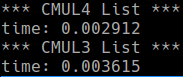
\includegraphics[width=0.3\textwidth]{time_sample.png}
                \caption{Sample Output of The Program Generated by cmplx\_numbers\_32\_008bit.txt} \label{time_sample}
            \end{center}
        \end{figure}

        The program, however, generates its output after a single iteration of the function call. The output times may vary on each execution due to the hosting machine fluctuating on its core and memory usage from other running processes. Therefore, further steps were taken to compute additional statistics on the timings.

        The sample input data consisted of integers of 8, 10, 20, 30, 40, 100, and 200 bits divided into 32 and 64 repetitions. An additional Makefile has been provided to generate timings on multiple iterations. 200 iterations were used to compute the current statistics. Furthermore, each iteration recompiles before running the program. A clean compilation prevents any external influences and overhead from the system on the individual timings. All the outputs for a single input are dumped to a buffer file, which is later parsed by an external helper script to generate the (1) means and (2) element-to-element differences.

        \clearpage
        \newpage
        \subsection{Results}
        The distribution of the element-to-element differences were plotted against the size of the input data. Outliers were excluded when generating the box plots. Data points residing above the x-axis indicate instances when \texttt{cmul4()} yielded slower runtimes than \texttt{cmul3()} (i.e. \texttt{cmul4()} - \texttt{cmul3()} < 0). The data points on the negative region represent instances when \texttt{cmul4()} - \texttt{cmul3()} > 0, indicating faster runtimes by \texttt{cmul4()} than \texttt{cmul3()}.

        \begin{figure}[ht]
            \begin{center}
                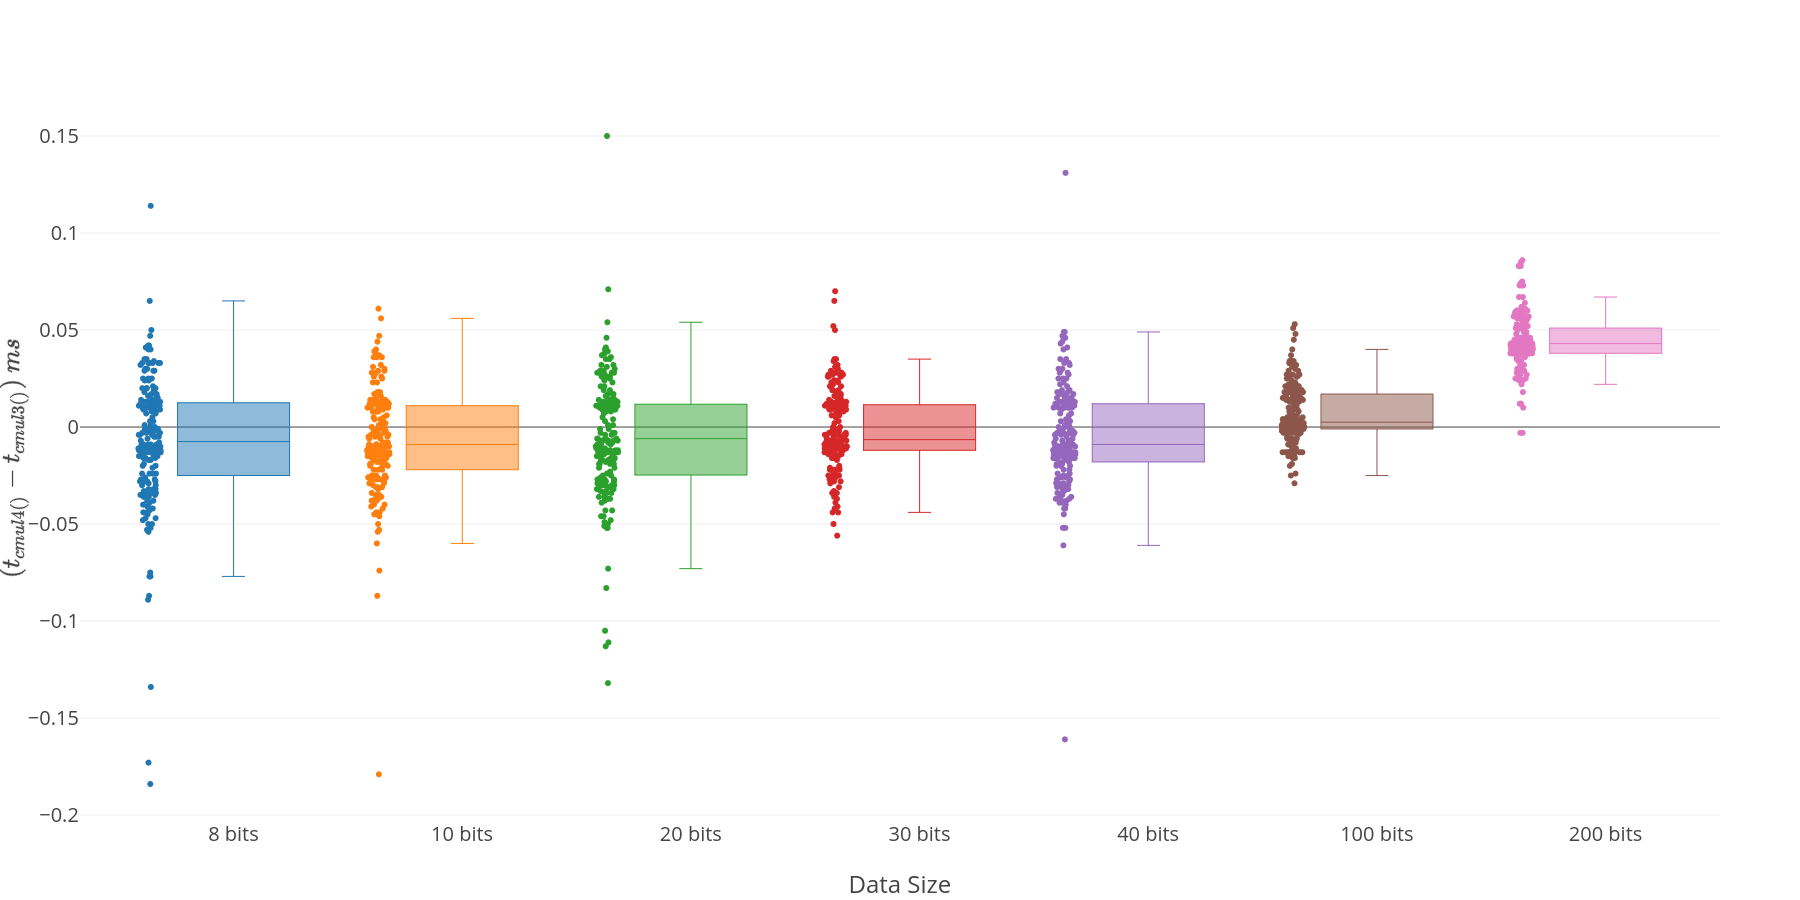
\includegraphics[width=0.9\textwidth]{32diffs.png}
                \caption{Distribution of Differences in The Multiplication Methods for n=32} \label{32diffs}
            \end{center}
        \end{figure}

        \begin{figure}[ht]
            \begin{center}
                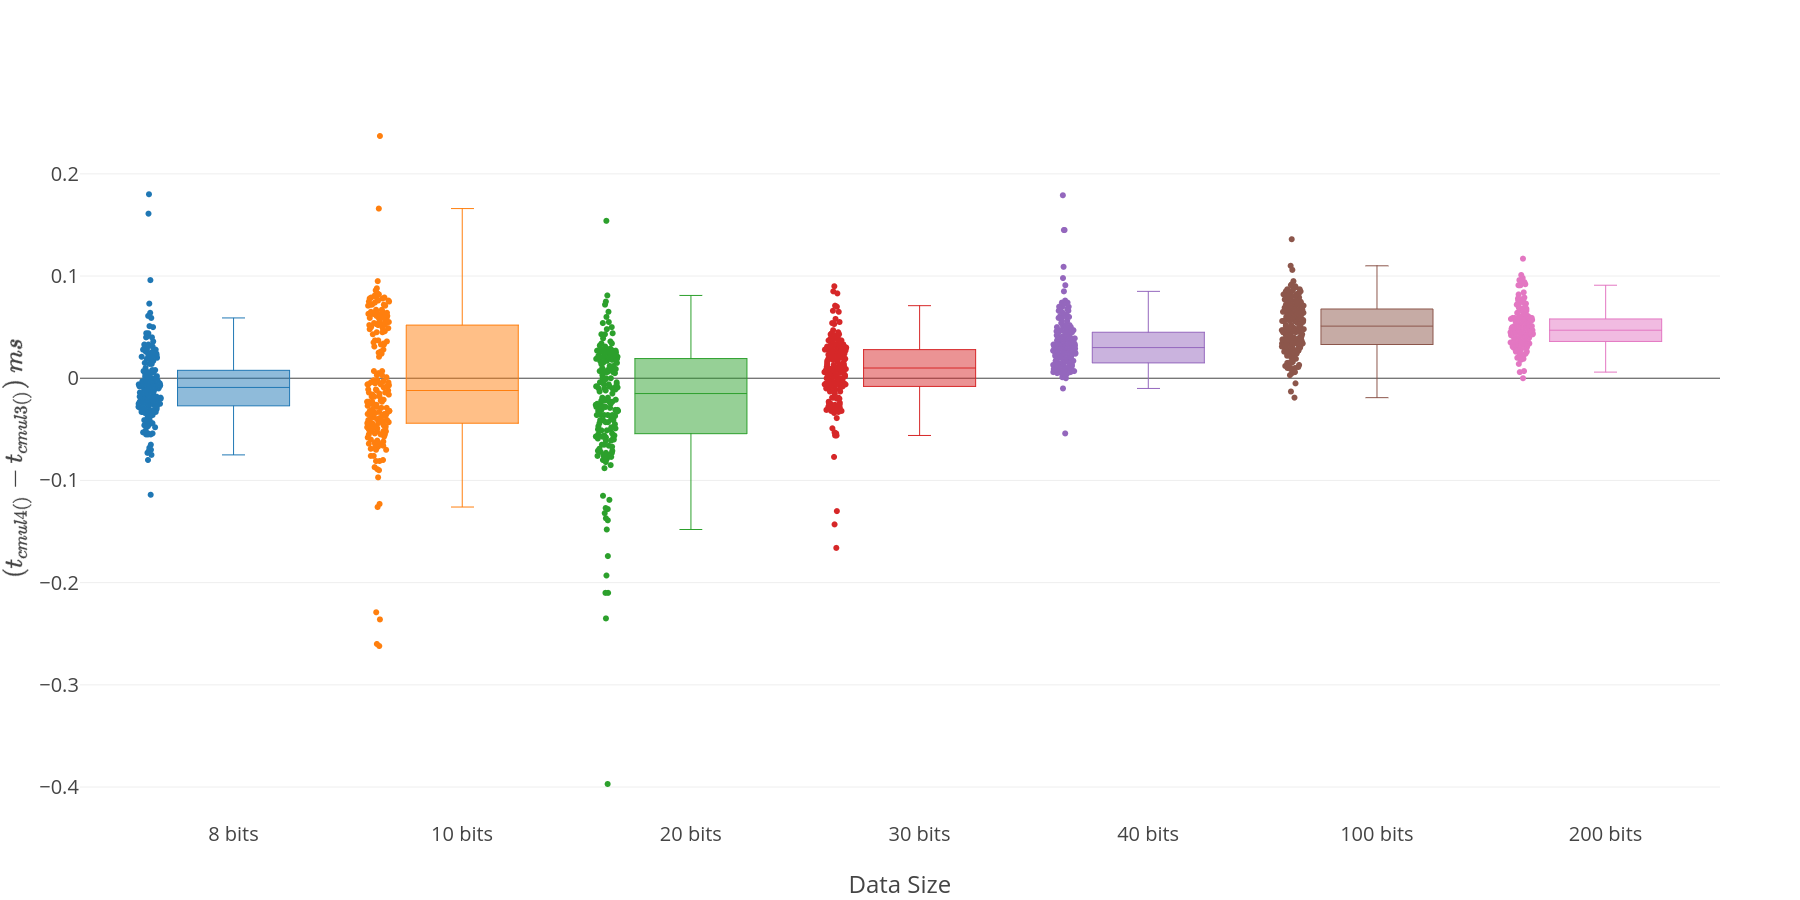
\includegraphics[width=0.9\textwidth]{64diffs.png}
                \caption{Distribution of Differences in The Multiplication Methods for n=64} \label{64diffs}
            \end{center}
        \end{figure}
        \clearpage
        \newpage

        The means of the times generated during testing were also plotted.
        \begin{figure}[ht]
            \begin{center}
                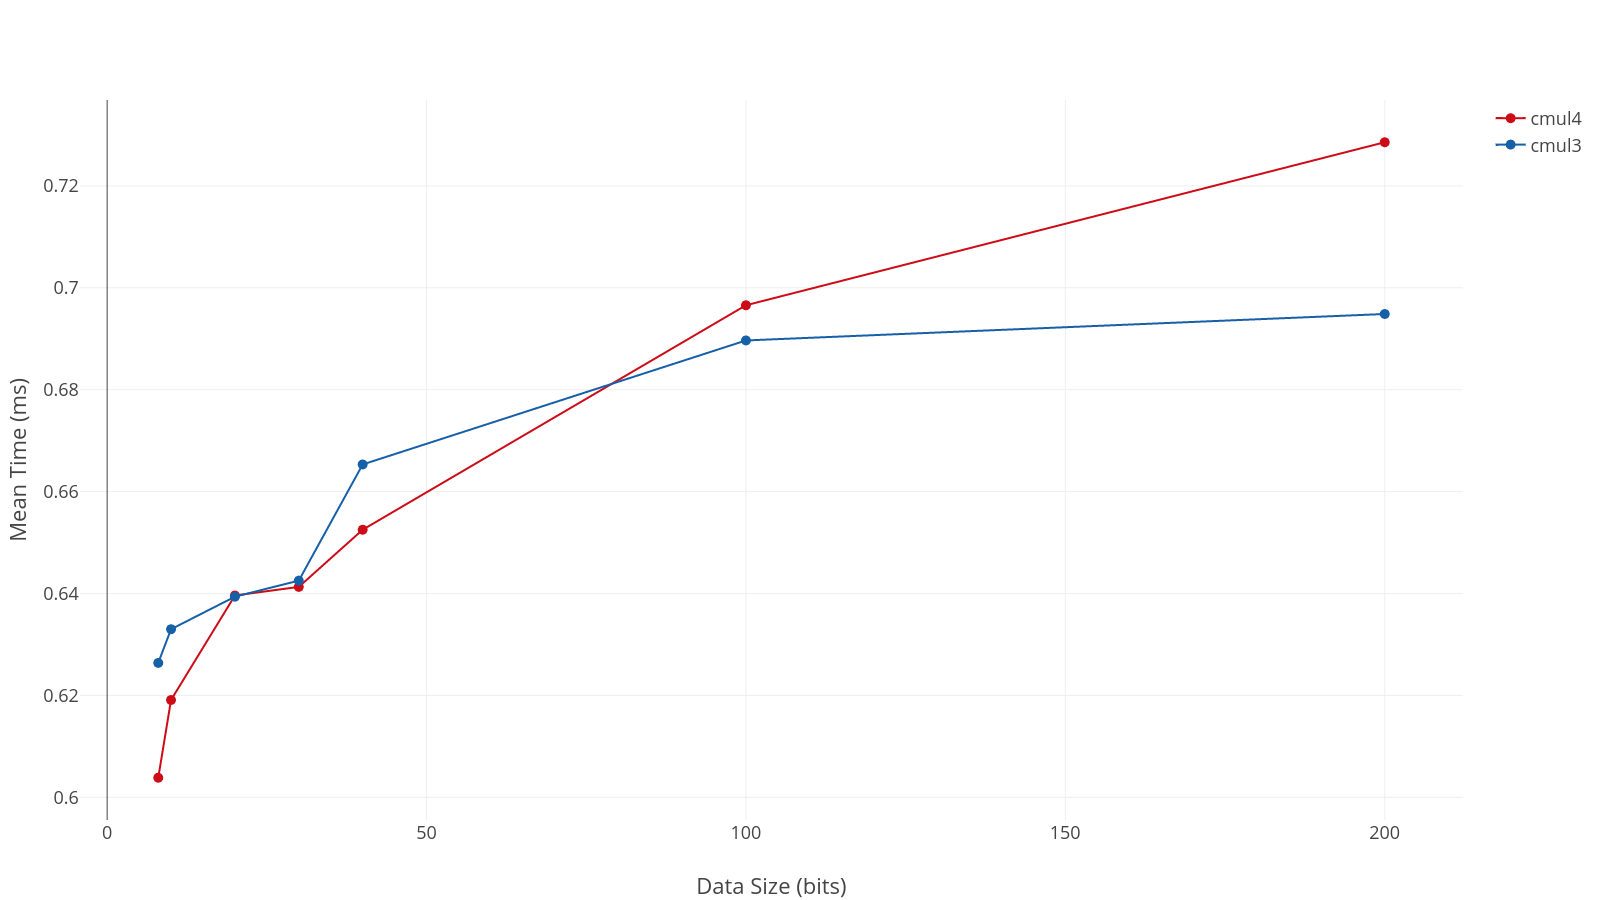
\includegraphics[width=0.80\textwidth]{32means.png}
                \caption{Means of The Multiplication Methods, with the Crossover Point $\epsilon$\texttt{[}75, 100\texttt{]} bits for n=32} \label{32diffs}
            \end{center}
        \end{figure}

        \begin{figure}[ht]
            \begin{center}
                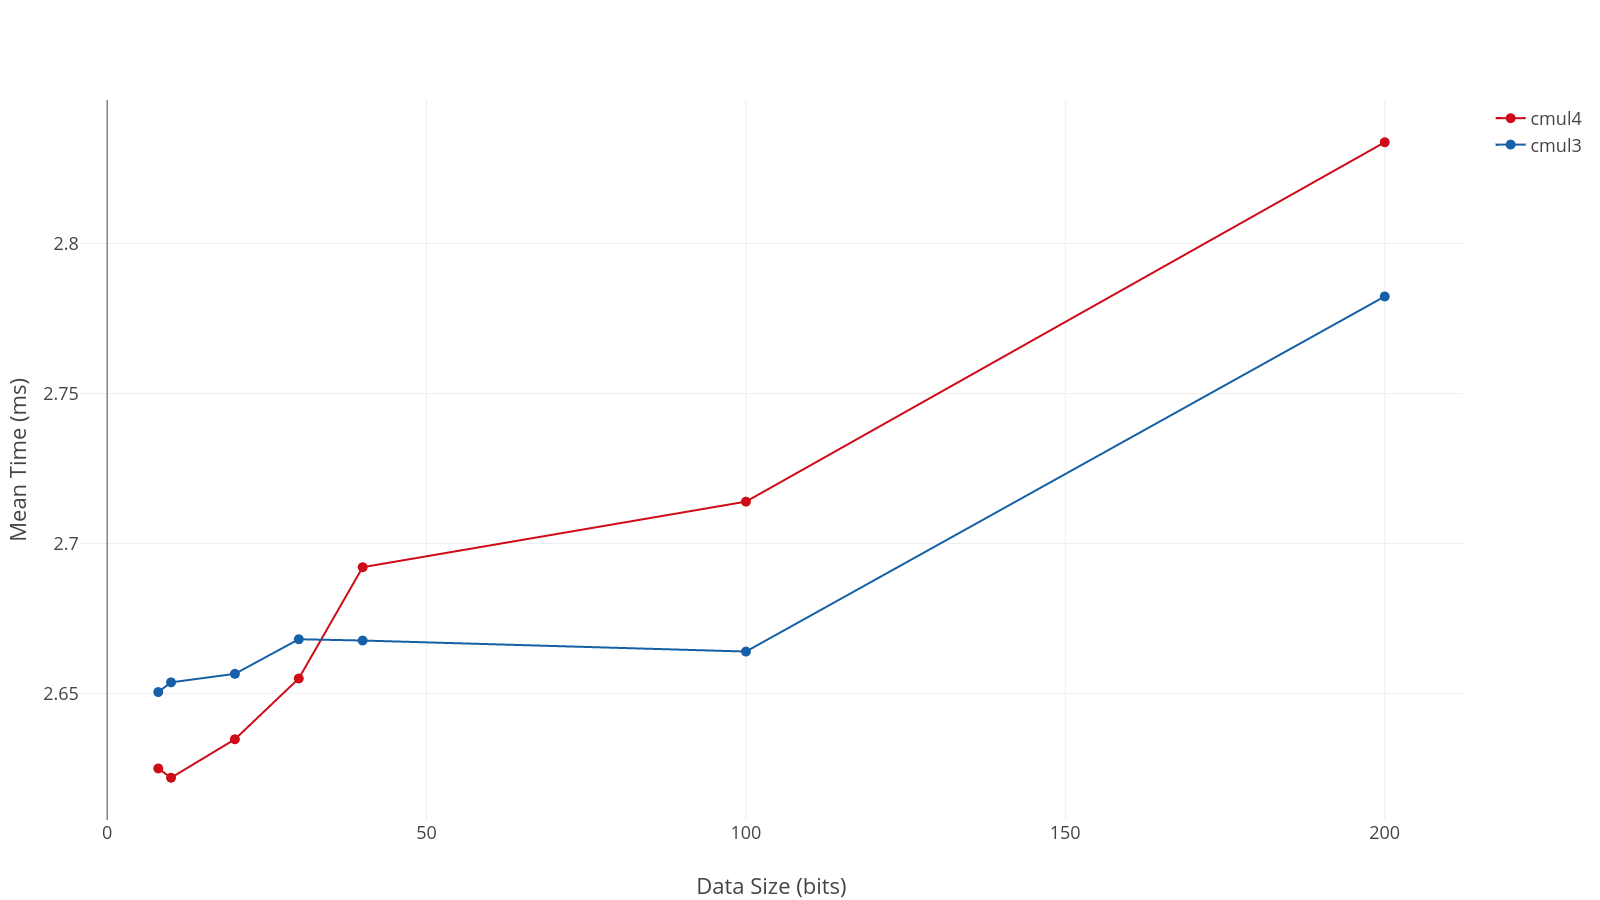
\includegraphics[width=0.80\textwidth]{64means.png}
                \caption{Means of The Multiplication Methods, with the Crossover Point $\epsilon$\texttt{[}40, 60\texttt{]} bits for n=64} \label{64diffs}
            \end{center}
        \end{figure}

        \clearpage
        \newpage
        \subsection{Troubleshooting}
        In the initial design of the source code, the execution times generated were being skewed by the implementation of the overloaded operators in the C++11 wrapper. The wrapper utilized an additional functionality that enabled the compiler to control the number of cores being used. Since the data were generated using a machine with 4 CPUs, this functionality appeared to generate faster execution times for larger input data. This functionality was removed from the system libraries, and the data were regenerated.

        These modifications did not require any changes to the source code since the initial design, but they were updated with minor modifications that do not affect the outputs.

\end{document}
